% Left: the graph of sqrt(1-x^2) is a quarter circle of area pi/4.
% Right: partial products of Wallis, climbing toward pi/2.
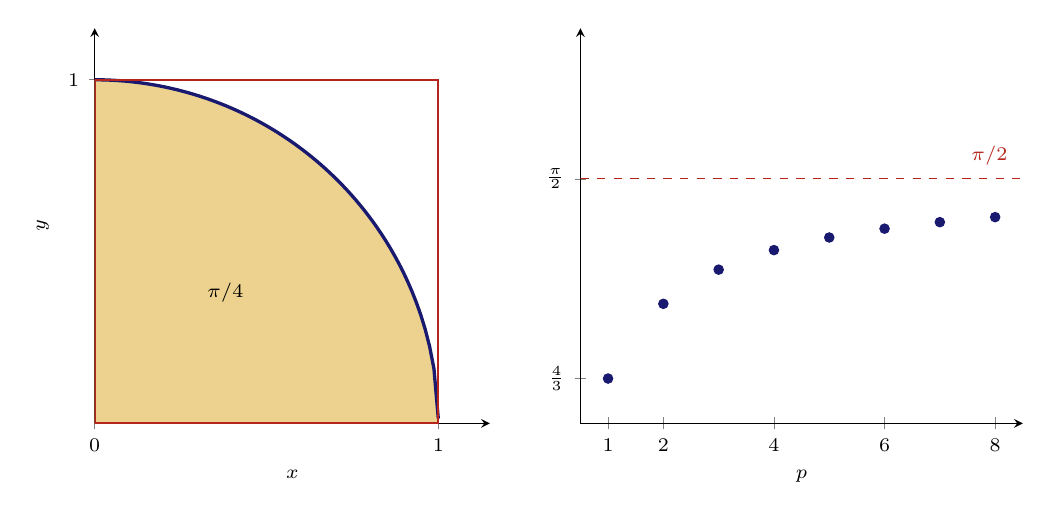
\begin{tikzpicture}
\begin{axis}[name=L,width=6.6cm,height=6.6cm,axis equal image,xmin=0,xmax=1.15,ymin=0,ymax=1.15,axis lines=left,xlabel={$x$},ylabel={$y$},xtick={0,1},ytick={1},tick label style={font=\scriptsize},label style={font=\scriptsize}]
  \addplot[draw=none,fill=Goldenrod!50,domain=0:1,samples=80] {sqrt(1-x*x)} \closedcycle;
  \addplot[MidnightBlue,very thick,domain=0:1,samples=80] {sqrt(1-x*x)};
  \draw[BrickRed,thick] (axis cs:0,0) rectangle (axis cs:1,1);
  \node[font=\scriptsize] at (axis cs:0.38,0.38) {$\pi/4$};
\end{axis}
\begin{axis}[at={(L.east)},anchor=west,xshift=1.15cm,width=7.2cm,height=6.6cm,xmin=0.5,xmax=8.5,ymin=1.28,ymax=1.75,axis lines=left,xlabel={$p$},ylabel={},xtick={1,2,4,6,8},ytick={1.333333,1.570796},yticklabels={$\frac43$,$\frac\pi2$},tick label style={font=\scriptsize},label style={font=\scriptsize}]
  \draw[BrickRed,dashed] (axis cs:0.5,1.570796) -- (axis cs:8.5,1.570796);
  \node[font=\scriptsize,BrickRed,anchor=south east] at (axis cs:8.4,1.575) {$\pi/2$};
  \addplot[MidnightBlue,only marks,mark=*,mark size=1.7pt] coordinates {(1,1.333333) (2,1.422222) (3,1.462857) (4,1.486077) (5,1.501088) (6,1.511585) (7,1.519337) (8,1.525295)};
\end{axis}
\end{tikzpicture}
